% English version of paper/ja_v4/04_結果.md (ver4, 2026-11-17). Subsection titles state conclusions (MIT CommLab results formula; Mensh & Kording rule 7); each paragraph ends with its answer. Sentences carried over from v3_04_analysis and v3_06_experiments with conditions called by name. Table 2: audio rows of the v3 gain table; Table 3: v3 Table 3(b); Table 4: counts per comparator (full table: Table S10). Figs. 3 and 5: paper/scripts/make_figs_v4.py.
\FloatBarrier
\section{Results}\label{sec:results}

\subsection{Audio classifiers retrained by distillation had higher UAR than the 11 methods that do not use pseudo-labels including other modalities}\label{sec:res-methods}
Table~\ref{tab:audiogain} gives the difference in UAR between audio classifiers retrained by distillation and the baseline. Audio UAR after distillation was higher than that of the baseline in all 12 conditions with four corpora and K = 5, 10 and 25, with intervals above zero in the nine conditions other than IEMOCAP (+2.71 to +4.15\pt). On IEMOCAP, the differences were +1.45 to +2.41\pt, with intervals including zero at all three K. Against the 11 methods that do not use pseudo-labels including other modalities, distillation was higher in all 132 comparisons over the 12 conditions, with intervals not above zero only in 10 comparisons on IEMOCAP (Fig.~\ref{fig:vsmethods}; K = 5 UARs in Table~S4). The version that uses the classifier's own baseline probabilities as pseudo-labels gave $-$1.0 to +0.5\pt\ relative to the baseline. For audio classifiers, pseudo-labels including other modalities gave higher UAR than the 11 methods that do not use them.

\begin{table}[!htbp]
\caption{Audio UAR after distillation was higher than that of the baseline in all 12 conditions with K = 5, 10 and 25, with intervals above zero in the nine other than IEMOCAP. Values: audio classifier retrained by distillation $-$ baseline (UAR points on test utterances) with 95\% intervals without correction, averaged over 50 repetitions (5 for K = 0). At K = 0, the baseline is the anchor (source only) and distillation uses no labels. K = 10 values follow an aggregation decided before the evaluation run (intervals only, no tests). IEMOCAP: improvised part. Visual, text and AVT classifiers: Table~S3}\label{tab:audiogain}
\footnotesize\setlength{\tabcolsep}{3.4pt}
\begin{tabular}{@{}lllll@{}}
\toprule
Corpus & K = 0 & K = 5 & K = 10 & K = 25 \\
\midrule
AFEW & +4.86 [+2.32, +7.40] & +4.15 [+2.56, +5.74] & +3.78 [+2.19, +5.38] & +3.32 [+1.40, +5.25] \\
IEMOCAP & +4.76 [+1.89, +7.63] & +2.41 [$-$0.45, +5.27] & +2.01 [$-$0.57, +4.58] & +1.45 [$-$0.48, +3.37] \\
MOSEI & +2.13 [+1.08, +3.19] & +3.19 [+2.38, +3.99] & +4.11 [+3.20, +5.01] & +3.36 [+2.56, +4.16] \\
MELD & +3.89 [+0.28, +7.51] & +3.12 [+1.18, +5.06] & +2.71 [+0.66, +4.77] & +2.86 [+1.21, +4.51] \\
\botrule
\end{tabular}
\end{table}

\begin{figure}[t]
\centering
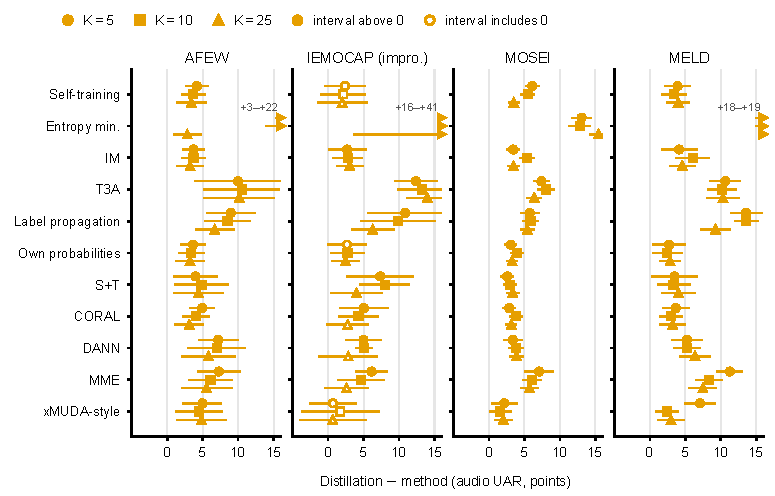
\includegraphics[width=\textwidth]{figures/fig_v4_methods_en.pdf}
\caption{Audio classifiers retrained by distillation had higher UAR than the 11 methods that do not use pseudo-labels including other modalities in all 132 comparisons. Points: distillation $-$ method (UAR points; four corpora $\times$ K = 5, 10, 25); lines: 95\% intervals without correction; open markers: intervals including zero (10 comparisons, all on IEMOCAP). Differences above 16\pt\ are drawn as right-pointing markers at the edge (in place of the K markers), with the method's range rounded to integers}\label{fig:vsmethods}
\end{figure}

Without labels (K = 0), the audio gain of distillation also had intervals above zero on all four corpora (+2.13 to +4.86\pt). The audio classifier retrained on pseudo-labels alone (K = 0) had higher UAR than the baseline with 5 and 10 labels per emotion on all four corpora (e.g.\ 53.4 vs 50.1 and 51.1 on AFEW; all values in Supplementary Information S2; no intervals computed). For audio classifiers, pseudo-labels including other modalities gave higher UAR than 5 or 10 labels per emotion.

By contrast, the gains of the visual, text and AVT classifiers varied across corpora (Table~S3). The gain of the text classifier on IEMOCAP was +5.01 to +7.34\pt, with intervals above zero at all three K, and its intervals included zero on the other corpora; visual intervals were above zero only for MOSEI at K = 10 and 25, and AVT intervals only for MELD at all K and MOSEI at K = 25. For AVT, the differences from the 10 methods other than the xMUDA-style method (which was not computed for AVT) were also mixed: some methods, such as self-training on AFEW (72.1 vs 70.8), were higher than distillation, and at K = 5 only CORAL on MOSEI was higher with the interval of the difference below zero. The 11 methods use information other than pseudo-labels including other modalities, so we read these differences as differences in the information used rather than in the quality of the methods.

\subsection{Pseudo-labels including other modalities reduced the error that remains after removing bias, which same-modality unlabelled utterances rarely did}\label{sec:res-remaining}
Table~\ref{tab:remaining} counts, in the all-source setting, the conditions in which distillation and the eight methods using same-modality unlabelled utterances reduced the remaining error (direction loss) relative to the baseline. Distillation reduced the remaining error in 38 of 81 conditions and increased it in one; its UAR was judged higher than the baseline (same rule) in 32 and lower in none. The eight methods reduced the remaining error in 7 of 210 conditions and increased it in 79. If the true differences were zero and conditions independent, the expected numbers of ``reduced'' conditions would be 2.02 and 5.25. Comparing point estimates on the same anchors and conditions (two modality groups, K = 0 and 5), distillation reduced the remaining error more in 341 of 373 pairs (pairs are not independent). In the all-source setting, the remaining error was reduced mainly by pseudo-labels including other modalities and rarely by same-modality unlabelled utterances.

\begin{table}[!htbp]
\caption{In the all-source setting, the remaining error (direction loss) was reduced in 38 of 81 conditions by distillation and in 7 of 210 by the eight methods using same-modality unlabelled utterances. Values: numbers of conditions by verdict. Direction loss: reduced / same level / increased / undetermined; UAR (method $-$ baseline): higher / same level / lower / undetermined. ``16 more'' are conditions in which the adaptation term of DANN or MME did not change predictions beyond seed variation (separate from the 48 undetermined). Visual direction losses come from features that failed the approximation check (Supplementary Information S2)}\label{tab:remaining}
\footnotesize
\begin{tabular}{@{}lllrll@{}}
\toprule
Method & Modalities & Classifier & Conditions & Direction loss$^{a}$ & UAR \\
\midrule
Distillation & A, V, T (3 corpora) & Audio & 9 & 9/0/0/0 & 9/0/0/0 \\
 &  & Visual & 9 & 1/1/0/7 & 1/0/0/8 \\
 &  & Text & 9 & 5/0/1/3 & 4/0/0/5 \\
 &  & AVT & 9 & 6/1/0/2 & 5/2/0/2 \\
 & A, V (5 corpora) & Audio & 15 & 7/0/0/8 & 7/0/0/8 \\
 &  & Visual & 15 & 5/0/0/10 & 4/1/0/10 \\
 &  & AV & 15 & 5/5/0/5 & 2/2/0/11 \\
\midrule
Distillation, total & & & 81 & 38/7/1/35 & 32/5/0/44 \\
Eight methods & Single modality & A, V, T & 210 & 7/60/79/48 (16 more) & --- \\
\botrule
\end{tabular}
\footnotetext{$^{a}$Halving $\delta$ gives 49 of 81 ``reduced'' conditions for distillation; doubling it gives 20}
\end{table}

\subsection{The more accurate the pseudo-labels were than the classifier before retraining, the higher the UAR after retraining}\label{sec:res-margin}
We related the advantage to the gain over the variants retrained with other pseudo-label providers (Sect.~\ref{sec:distill}). For example, on MOSEI with K = 25, retraining the audio classifier on pseudo-labels from the visual--text classifier gave an advantage of +4.6\pt\ (42.2 vs 37.6) and a gain of +2.05 [+0.74, +3.35]\pt. On AFEW with K = 5, retraining the visual classifier on pseudo-labels from the audio--text classifier gave an advantage of $-$16.7\pt\ (54.4 vs 71.1) and a gain of $-$4.40 [$-$7.70, $-$1.09]\pt.

Over the 360 variants, the ranks of advantage and gain agreed: the rank correlation was 0.80 at K = 5 and 0.83 at K = 25, and within each of the 32 combinations of corpus, retrained classifier and K it was positive (median 0.92, minimum 0.39). Figure~\ref{fig:margincounts} counts the variants by the sign of the advantage and the gain interval. No variant with a negative advantage (173 at K = 5, 184 at K = 25) had a gain interval above zero, and 125 and 144 had intervals below zero. Among variants with a positive advantage (187 and 176), 58 and 42 had intervals above zero, while 16 and 20 had intervals below zero (breakdown in Supplementary Information S2). Of the 360 variants counted, every variant whose UAR rose had pseudo-labels more accurate than the classifier before retraining (the one excluded variant whose advantage is zero by construction rose; Supplementary Information S2).

\begin{figure}[t]
\centering
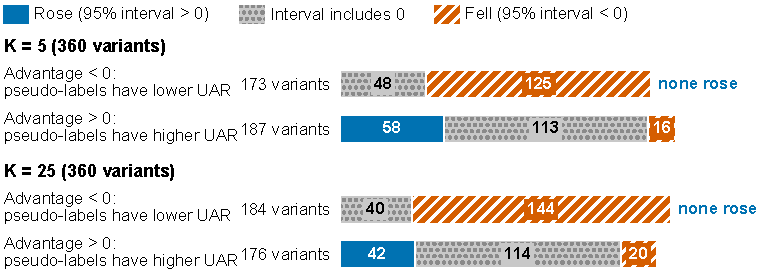
\includegraphics[width=\textwidth]{figures/fig_margin_counts_en.pdf}
\caption{No variant whose pseudo-labels were less accurate than the classifier before retraining (negative advantage) rose (gain interval above zero). Variants retrained with other pseudo-label providers (360 per K; K = 5 and 25) counted by the sign of the advantage and by the 95\% interval of the gain (above zero, including zero, below zero). One variant is one combination of corpus, retrained classifier and pseudo-label provider; the gain is the difference in test UAR}\label{fig:margincounts}
\end{figure}

Among unimodal classifiers, the one whose baseline had the highest candidate UAR (hereafter the corpus's strongest modality) was visual on AFEW, audio on IEMOCAP, visual on MOSEI and text on MELD at both K = 5 and 25. Retraining the classifier of the strongest modality on pseudo-labels from the classifier on the concatenated features of the other two modalities gave negative gains in point estimates in all eight cases (four corpora and two K; $-$4.40 to $-$1.02\pt). The classifier of the strongest modality had lower UAR than before retraining, in point estimates, when it was retrained on pseudo-labels from the other two modalities alone.

\subsection{Predictions fused by the proposal had higher UAR than the equal-weight product in 11 of 12 conditions}\label{sec:res-prop}
Figure~\ref{fig:propfig}(a) shows the difference in UAR between the proposal and the product, and Table~\ref{tab:propcount} counts, for each way of combining the three classifiers' predictions, the signs and intervals of the differences from the proposal (UARs and differences in Table~S10). The fused predictions are the argmax of the combined predictions of the three classifiers on test utterances, without retraining any classifier. Proposal $-$ product was positive in 11 of 12 conditions, with 95\% intervals excluding zero in seven (AFEW at all K, IEMOCAP and MOSEI at K = 25, MELD at K = 10 and 25). The largest differences were on AFEW (+2.13 to +3.51\pt). On AFEW, the visual product component's UAR exceeded the audio and text components by more than 17\pt\ (K = 5: visual 70.70, audio 53.24, text 45.76), and the visual classifier alone was higher than the product at K = 5 and 10 (70.70 vs 69.23, 71.93 vs 70.88). On IEMOCAP, MOSEI and MELD, proposal $-$ product ranged from $-$0.09 to +0.83\pt\ over the nine conditions. The difference from the probability mean was positive in 8 of 12 conditions, with intervals above zero on AFEW at all K and MOSEI at K = 25 and none below zero. The proposal made more accurate predictions than the equal-weight product in 11 of 12 conditions and than the probability mean in 8.

\begin{table}[!htbp]
\caption{The proposal had higher UAR than every comparator in at least 8 of 12 conditions; intervals lay below zero (proposal lower) in only one condition against temperature calibration and two against the version without strength differences. Values: counts over 4 corpora $\times$ K = 5, 10, 25 of the difference proposal $-$ comparator (for retrained AVT: AVT retrained on the proposal's pseudo-labels $-$ comparator), with 95\% intervals without correction. The strongest single classifier was added after the evaluation run (Sect.~\ref{sec:protocol}). UARs and differences per condition: Table~S10; CREMA-D (audio and visual): Table~S8}\label{tab:propcount}
\footnotesize
\begin{tabular}{@{}p{4.5cm}cccl@{}}
\toprule
Comparator & Positive & Interval above 0 & Interval below 0 & Range (points) \\
\midrule
\multicolumn{5}{@{}l}{\textit{Fused predictions}} \\
Product (equal weights) & 11 & 7 & 0 & $-$0.09 to +3.51 \\
Probability mean & 8 & 4 & 0 & $-$0.49 to +3.73 \\
Per-classifier temperature calibration & 8 & 4 & 1 & $-$2.94 to +1.18 \\
Strongest single classifier on the K labels & 12 & 7 & 0 & +2.70 to +5.52 \\
Proposal without per-emotion profiles & 12 & 5 & 0 & +0.10 to +0.73 \\
Proposal without strength differences & 8 & 3 & 2 & $-$0.42 to +3.20 \\
\multicolumn{5}{@{}l}{\textit{Retrained AVT}} \\
Baseline AVT & 10 & 7 & 0 & $-$0.56 to +3.05 \\
AVT retrained on the product's pseudo-labels & 11 & 5 & 0 & $-$0.05 to +1.95 \\
\botrule
\end{tabular}
\end{table}

\begin{figure}[t]
\centering
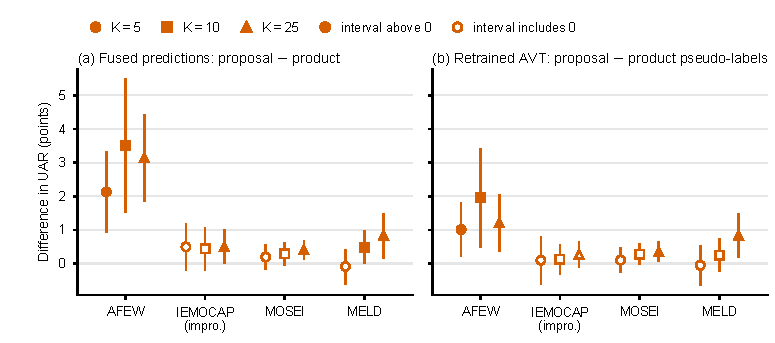
\includegraphics[width=\textwidth]{figures/fig_v4_prop_en.pdf}
\caption{Predictions fused by the proposal had higher UAR than the equal-weight product, and AVT classifiers retrained on the proposal's pseudo-labels had higher UAR than those retrained on the product's pseudo-labels, each in 11 of 12 conditions, with the largest differences on AFEW. (a) Fused predictions: proposal $-$ product. (b) AVT retrained on the proposal's pseudo-labels $-$ AVT retrained on the product's pseudo-labels. Points: differences; lines: 95\% intervals without correction; open markers: intervals including zero}\label{fig:propfig}
\end{figure}

By contrast, differences from comparators that fit to the few labels or select one classifier depended on the comparator. Against per-classifier temperature calibration (inverse temperatures fitted to the K-label log-likelihood \cite{guo2017calibration}; three quantities fitted on the K labels, as in the proposal), the difference was positive in 8 of 12 conditions, and the proposal was lower with the interval excluding zero only on AFEW at K = 5 ($-$2.94 [$-$5.6, $-$0.3], 71.36 vs 74.30). Against the single classifier with the highest K-label strength, the proposal was higher in all 12 conditions (+2.70 to +5.52\pt), with intervals above zero in seven (IEMOCAP at K = 5, MOSEI and MELD at all K). Decomposing the difference, multiplying the three classifiers' predictions (product $-$ strongest single: +2.04 to +5.02\pt) accounted for most of it on IEMOCAP, MOSEI and MELD, and changing the weights (proposal $-$ product) accounted for most of it on AFEW (details in Supplementary Information S5). Comparisons with seven further combinations are in Supplementary Information S6.

\subsection{Removing strength differences lowered UAR on AFEW, and removing per-emotion profiles lowered UAR on MOSEI}\label{sec:res-ablation}
We compared the proposal with versions without one of its parts (Table~\ref{tab:propcount}; Table~S10). On MOSEI, the difference from the proposal without per-emotion profiles had intervals above zero at all K (+0.51 to +0.73\pt), and so did CREMA-D (Supplementary Information S7). On AFEW, the difference from the proposal without strength differences had intervals above zero at all K (+1.74 to +3.20\pt), accounting for most of AFEW's proposal $-$ product (+2.13 to +3.51\pt). On MOSEI at K = 5 and 10, by contrast, the version without strength differences had higher UAR ($-$0.42 [$-$0.7, $-$0.1] and $-$0.35 [$-$0.6, $-$0.1]\pt). Counted after the evaluation over its 50 repetitions, the classifier with the highest K-label strength was the classifier with the highest strength on all candidate labels (visual on AFEW, audio on IEMOCAP, text on MELD) in 0.70--1.00 of repetitions, whereas the classifier with the highest source-measured strength was a different classifier on all three corpora. On MOSEI, where the top two strengths were close, this fraction was 0.30--0.38 (values per corpus and K in Supplementary Information S5). Strength differences raised the proposal's UAR on AFEW, where the visual classifier's UAR exceeded those of the audio and text classifiers by more than 17\pt, and per-emotion profiles raised it on MOSEI, where the strongest modality changed with the emotion.

\subsection{AVT classifiers retrained on the proposal's pseudo-labels also had higher UAR than those retrained on the product's pseudo-labels in 11 of 12 conditions}\label{sec:res-retrain}
We retrained the AVT classifier on the proposal's pseudo-labels (Fig.~\ref{fig:propfig}(b); lower part of Table~\ref{tab:propcount}). Its UAR was higher than that of the AVT retrained on the product's pseudo-labels in 11 of 12 conditions, with intervals above zero in five (AFEW at all K, MOSEI and MELD at K = 25; +1.01, +1.95 and +1.21\pt\ on AFEW); the other nine differences ranged from $-$0.05 to +0.82\pt. Against the baseline AVT, the difference was positive in 10 of 12 conditions and above zero in seven. On CREMA-D (audio and visual), proposal $-$ product of the fused predictions and AV retrained on the proposal's pseudo-labels $-$ AV retrained on the product's pseudo-labels were +0.31 to +0.63\pt, with all six intervals excluding zero (Supplementary Information S7). Classifiers retrained on the proposal's pseudo-labels, whose fused predictions were more accurate than the product, also had higher UAR than those retrained on the product's pseudo-labels.
